\section{What the forecast is for}
\label{sec:sizing}

A predicted standard deviation is not a result on its own. Nobody trains a model in order to learn
how much its score would move under a different seed; they want to know whether one recipe beats
another, and the deviation is what says how many runs settle it.

\subsection{The decision}

Two configurations are to be ordered. A practitioner trains each for a seed, looks at the lead, and
either calls it or trains another seed of each. Stopping when the lead $\bar D_k$ after $k$ seeds
per arm clears $z$ standard errors,
\begin{equation}
  \label{eq:stop}
  |\bar D_k| \;\ge\; z\,\frac{\sigma_D}{\sqrt{k}},
  \qquad
  \sigma_D=\sqrt{\sigma_A^2+\sigma_B^2},
\end{equation}
is the rule this instantiates. It needs $\sigma_D$, and that is the difficulty: at $k=1$ there is no
empirical deviation to put there. The remaining choices are to fix $k$ in advance, which is what is
normally done, or to spend seeds building a variance estimate before the comparison can begin.
Sections~\ref{sec:theory} and \ref{sec:estimation} supply $\sigma_A$ and $\sigma_B$ from the first
run of each arm, so \eqref{eq:stop} is available from $k=1$.

Note what \eqref{eq:stop} does \emph{not} require. Multiplying every $\sigma$ by a common factor is
undone by dividing $z$ by the same factor, so a forecast uniformly off by a constant reaches the
same operating points as one that is not, provided $z$ ranges widely enough to allow the move. What
matters is the \emph{relative} deviation across configurations.

\subsection{Setup}

The scores are the $\numSizeSeeds$ per-seed scores already stored for each of the $\numSizeArms$
configurations of Section~\ref{sec:forecast}; no new training is done, and every policy sees the
same seeds in the same order, so the comparison is paired. We compare configurations sharing a
task.

The true ordering has to come from somewhere, and reading it from seeds a policy is also shown
would correlate the policy's evidence with the answer it is graded against, flattering whichever
policy looks at the most seeds. So $\numSizeHoldout$ of the $\numSizeSeeds$ seeds are reserved: the
ordering is fixed on those and no policy may draw one. The $\numSizePairs$ pairs whose
reserved-seed ordering is unambiguous at four standard errors are kept, so a disagreement is a
mistake rather than a coin landing the other way up, and policies draw from the remaining
$\numSizeCap$. Each pair is replayed under $400$ random orderings.

A policy is a curve rather than a point, since $z$ trades runs against mistakes, and reading every
curve at a common mistake rate is what makes two comparable. We report the runs each needs to hold
its mistake rate at $\numSizeTarget\%$, both arms counted.

\begin{table}[t]
  \centering \small
  \begin{tabular}{lccc}
  \toprule
  policy & runs & vs.\ adjoint & $95\%$ \\
  \midrule
    fixed budget, no stopping rule & 30.41 & $9.57$ & $[7.24, 10.56]$ \\
    deviation from the seeds in hand & 6.52 & $2.13$ & $[1.98, 2.38]$ \\
    one deviation for every recipe & 6.04 & $1.93$ & $[1.45, 2.28]$ \\
    frozen forecast, before any run & 3.34 & $1.09$ & $[1.02, 1.14]$ \\
    adjoint forecast, from one run & 3.07 & $1.00$ & $[1.00, 1.00]$ \\
    measured deviation & 3.16 & $1.02$ & $[0.99, 1.05]$ \\
  \bottomrule
\end{tabular}
  \caption{Runs needed to hold the mistake rate at $\numSizeTarget\%$ over $\numSizePairs$
  comparisons, both arms counted, with $95\%$ intervals from resampling the comparisons. The
  forecast is not better than knowing the deviation; it is not measurably worse, which is the
  point.}
  \label{tab:sizing}
\end{table}

\begin{figure}[t]
  \centering
  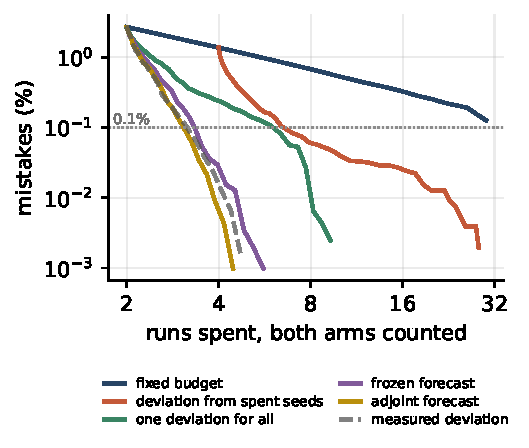
\includegraphics[width=\columnwidth]{sizing.pdf}
  \caption{Mistakes against runs spent. A policy is a curve, not a point, since the stopping
  threshold trades one against the other, and what separates two policies is how far left a curve
  sits at a fixed height. At $\numSizeTarget\%$ the forecasts cross near $\numSizeAdjointRuns$ runs
  and a fixed budget near $\numSizeFixedRuns$. The rule driven by spent seeds flattens on the left
  because it cannot stop before two seeds per arm however large the lead.}
  \label{fig:sizing}
\end{figure}

\subsection{Result}

The adjoint forecast reaches $\numSizeAdjointRuns$ runs and the ceiling, a rule handed the realised
deviation, reaches $\numSizeOracleRuns$: the same policy to within resampling error, at
$\numSizeOracleGain\times$ $[\numSizeOracleLo, \numSizeOracleHi]$. Fixed-budget practice needs
$\numSizeFixedRuns$ runs for the same reliability, $\numSizeFixedGain\times$
$[\numSizeFixedLo, \numSizeFixedHi]$ more. Estimating the deviation from spent seeds costs
$\numSizeEmpiricalGain\times$ $[\numSizeEmpiricalLo, \numSizeEmpiricalHi]$, and most of that is
structural rather than statistical: that rule cannot stop at one seed per arm however large the
lead, so four runs are committed before any comparison can be decided.

Grading against all $\numSizeSeeds$ seeds instead, so a policy's own seeds are part of the answer,
cuts the advantage over a fixed budget to $\numSizeOverlapFixed\times$. The overlap helps a policy
in proportion to how many seeds it draws, so it favours the baselines that draw the most, and the
headline numbers are the ones without it.

Note which predictor does the work. The frozen forecast \eqref{eq:frozen} uses the step size, the
run length and the two noise traces, with no stored trajectory and no backward pass. It reaches
$\numSizeFrozenRuns$ runs, within $\numSizeFrozenGain\times$ of the adjoint and still
$\numSizeFrozenVsFixed\times$ better than a fixed budget. The bulk of the saving does not require
Theorem~\ref{thm:adjoint} at all, and the backward pass buys the last $\numSizeFrozenGain\times$.
That is the cheap half a practitioner would deploy first.

\subsection{The other decision, where it helps less}

Sizing is not the only use of a deviation. The other is choosing: run each of several
configurations once and keep the one with the most gain per unit of noise and rollout. Reporting
only the decision that flatters the forecast would misrepresent it, so we measure both on the same
grid, with seeds split three ways and never reused across roles. One pilot supplies the observed
gain, a disjoint pool supplies whatever deviation a policy is entitled to, and a third reserved set
scores the choice. That last separation matters: letting the scoring seeds also set the deviation
makes an oracle look unbeatable, since its denominator then shares noise with the one it is graded
against, and an earlier version of this experiment did exactly that.

Over $\numPickTasks$ tasks the share of the best achievable value the choice keeps is
$\numPickConstant\%$ with one deviation for every recipe, $\numPickFrozen\%$ frozen,
$\numPickAdjoint\%$ adjoint and $\numPickOracle\%$ with the measured deviation: the forecast
recovers $\numPickGain$ points $[\numPickGainLo, \numPickGainHi]$ of the
$\numPickOraclePoints$ available, a share of $\numPickShare$.

The forecast is close to the ceiling in both decisions, but the ceilings differ. Choosing has only
$\numPickOraclePoints$ points of headroom at all, because a single pilot's observed gain is noisy
and that noise limits the choice whatever denominator is used. Sizing has no competing term: the
run count scales as $(\sigma/\mu)^2$, the deviation enters squared, and at one run per arm there is
no alternative estimate of it. That asymmetry, not the quality of the forecast, is why the two
numbers differ, and it is why we lead with sizing.

\subsection{How wrong the forecast may be}

On a pretrained model the forecast is accurate only in some regimes (Section~\ref{sec:real}), so we
corrupt it on purpose and rerun the benchmark: a lognormal multiplicative error of controlled
median magnitude, and separately a systematic scale error.

The scale error does nothing. Over $\numTolScaleRange$ orders of magnitude the runs needed change
by a factor of $\numTolScaleSpread$, because $z$ absorbs it exactly as \eqref{eq:stop} says. A
forecast used this way does not need to be calibrated, which is worth stating because it is the
opposite of what reporting an error bar requires.

Relative error is what costs. Runs needed rise from $\numTolClean$ at the measured accuracy to
$\numTolRunsOneHalf$ at a median error of $1.5\times$, $\numTolRunsDouble$ at $2\times$ and
$\numTolRunsTwoHalf$ at $2.5\times$, reaching the fixed budget's $\numTolFixed$ at about
$\numTolBreakeven\times$. The tolerance is wide but not unlimited: a forecast wrong by less than
roughly a factor of three pays for itself, and one wrong by twenty-five does not. That break-even
is the honest statement of scope, and Section~\ref{sec:real} is where it is tested.
